%!TeX root=../wowtop.tex

\ArtChapter[The Days of Imprisonment]{20head}

\lettrine[lines=4,findent=2pt]{T}{he} arrival of a second fighting-machine drove us from our peephole into the scullery, for we feared that from his elevation the Martian might see down upon us behind our barrier. At a later date we began to feel less in danger of their eyes, for to an eye in the dazzle of the sunlight outside our refuge must have been blank blackness, but at first the slightest suggestion of approach drove us into the scullery in heart-throbbing retreat. Yet terrible as was the danger we incurred, the attraction of peeping was for both of us irresistible. And I recall now with a sort of wonder that, in spite of the infinite danger in which we were between starvation and a still more terrible death, we could yet struggle bitterly for that horrible privilege of sight. We would race across the kitchen in a grotesque way between eagerness and the dread of making a noise, and strike each other, and thrust and kick, within a few inches of exposure.

\begin{figure}[tb]
\centering
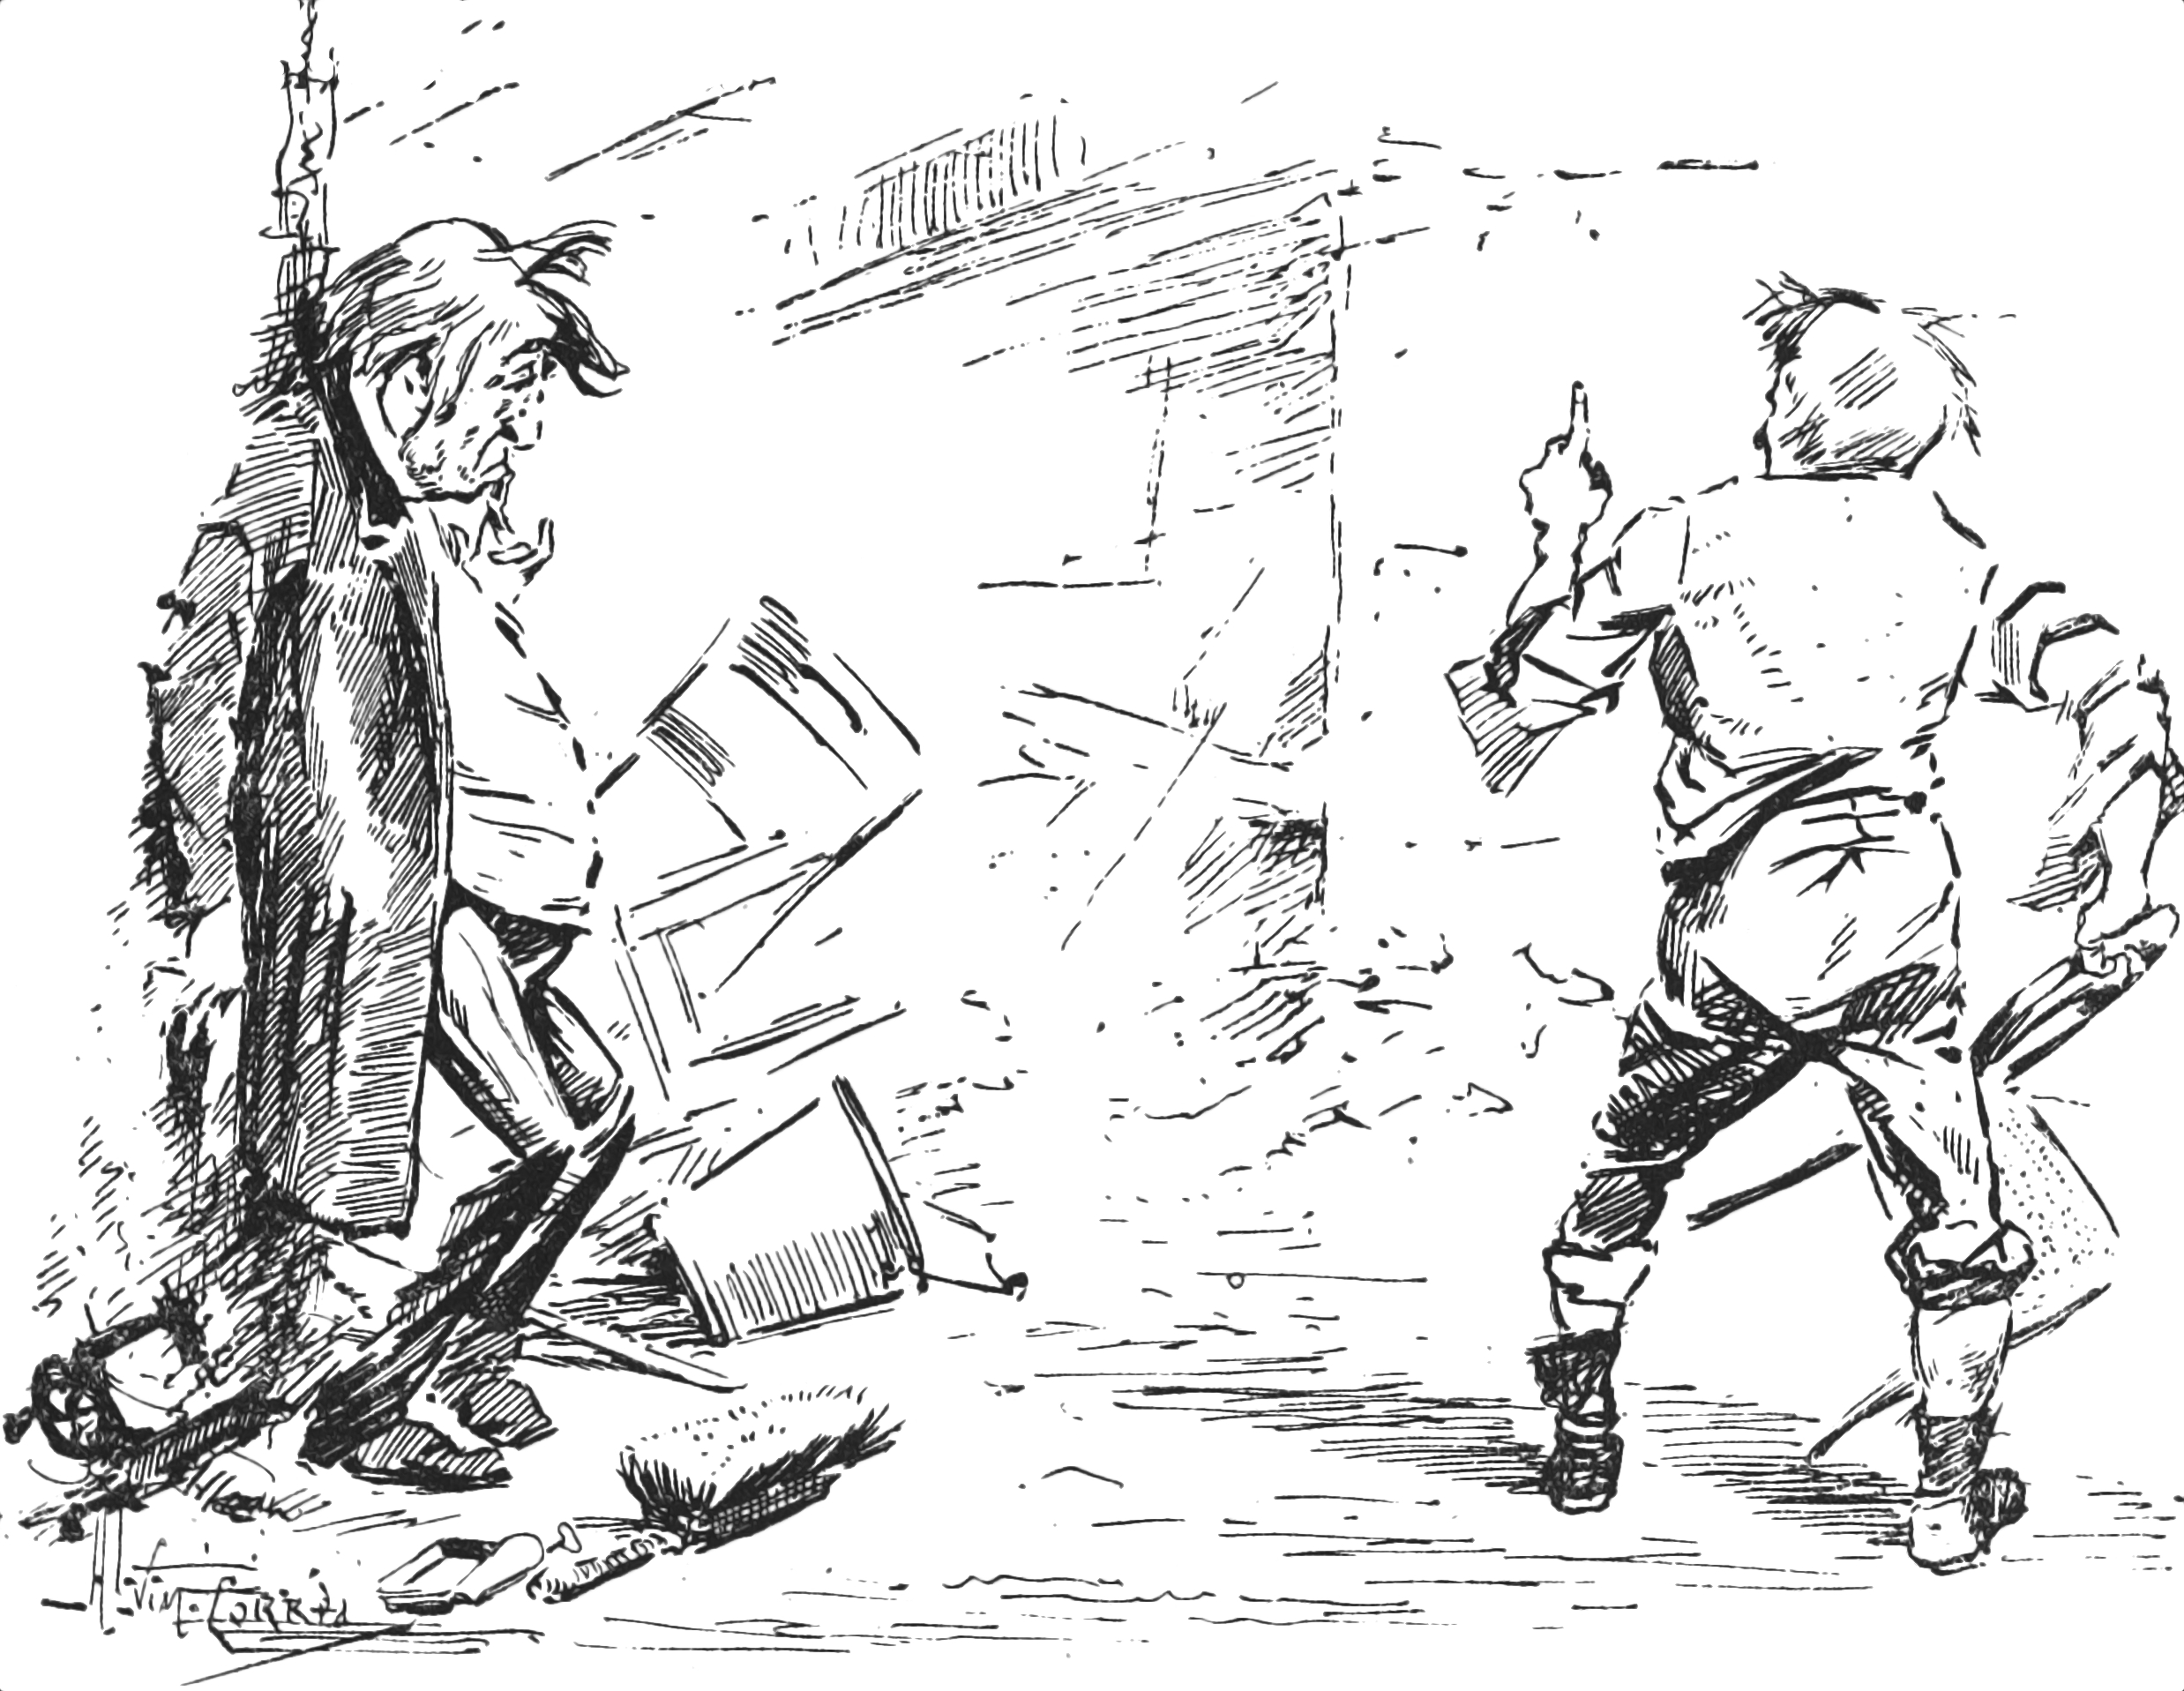
\includegraphics[width=.8\linewidth]{20defeated}
\end{figure}

The fact is that we had absolutely incompatible dispositions and habits of thought and action, and our danger and isolation only accentuated the incompatibility. At Halliford I had already come to hate the curate's trick of helpless exclamation, his stupid rigidity of mind. His endless muttering monologue vitiated every effort I made to think out a line of action, and drove me at times, thus pent up and intensified, almost to the verge of craziness. He was as lacking in restraint as a silly woman. He would weep for hours together, and I verily believe that to the very end this spoiled child of life thought his weak tears in some way efficacious. And I would sit in the darkness unable to keep my mind off him by reason of his importunities. He ate more than I did, and it was in vain I pointed out that our only chance of life was to stop in the house until the Martians had done with their pit, that in that long patience a time might presently come when we should need food. He ate and drank impulsively in heavy meals at long intervals. He slept little.

As the days wore on, his utter carelessness of any consideration so intensified our distress and danger that I had, much as I loathed doing it, to resort to threats, and at last to blows. That brought him to reason for a time. But he was one of those weak creatures, void of pride, timorous, anæmic, hateful souls, full of shifty cunning, who face neither God nor man, who face not even themselves.

It is disagreeable for me to recall and write these things, but I set them down that my story may lack nothing. Those who have escaped the dark and terrible aspects of life will find my brutality, my flash of rage in our final tragedy, easy enough to blame; for they know what is wrong as well as any, but not what is possible to tortured men. But those who have been under the shadow, who have gone down at last to elemental things, will have a wider charity.

And while within we fought out our dark, dim contest of whispers, snatched food and drink, and gripping hands and blows, without, in the pitiless sunlight of that terrible June, was the strange wonder, the unfamiliar routine of the Martians in the pit. Let me return to those first new experiences of mine. After a long time I ventured back to the peephole, to find that the new-comers had been reinforced by the occupants of no fewer than three of the fighting-machines. These last had brought with them certain fresh appliances that stood in an orderly manner about the cylinder. The second handling-machine was now completed, and was busied in serving one of the novel contrivances the big machine had brought. This was a body resembling a milk can in its general form, above which oscillated a pear-shaped receptacle, and from which a stream of white powder flowed into a circular basin below.

The oscillatory motion was imparted to this by one tentacle of the handling-machine. With two spatulate hands the handling-machine was digging out and flinging masses of clay into the pear-shaped receptacle above, while with another arm it periodically opened a door and removed rusty and blackened clinkers from the middle part of the machine. Another steely tentacle directed the powder from the basin along a ribbed channel towards some receiver that was hidden from me by the mound of bluish dust. From this unseen receiver a little thread of green smoke rose vertically into the quiet air. As I looked, the handling-machine, with a faint and musical clinking, extended, telescopic fashion, a tentacle that had been a moment before a mere blunt projection, until its end was hidden behind the mound of clay. In another second it had lifted a bar of white aluminium into sight, untarnished as yet, and shining dazzlingly, and deposited it in a growing stack of bars that stood at the side of the pit. Between sunset and starlight this dexterous machine must have made more than a hundred such bars out of the crude clay, and the mound of bluish dust rose steadily until it topped the side of the pit.

The contrast between the swift and complex movements of these contrivances and the inert panting clumsiness of their masters was acute, and for days I had to tell myself repeatedly that these latter were indeed the living of the two things.

The curate had possession of the slit when the first men were brought to the pit. I was sitting below, huddled up, listening with all my ears. He made a sudden movement backward, and I, fearful that we were observed, crouched in a spasm of terror. He came sliding down the rubbish and crept beside me in the darkness, inarticulate, gesticulating, and for a moment I shared his panic. His gesture suggested a resignation of the slit, and after a little while my curiosity gave me courage, and I rose up, stepped across him, and clambered up to it. At first I could see no reason for his frantic behaviour. The twilight had now come, the stars were little and faint, but the pit was illuminated by the flickering green fire that came from the aluminium-making. The whole picture was a flickering scheme of green gleams and shifting rusty black shadows, strangely trying to the eyes. Over and through it all went the bats, heeding it not at all. The sprawling Martians were no longer to be seen, the mound of blue-green powder had risen to cover them from sight, and a fighting-machine, with its legs contracted, crumpled, and abbreviated, stood across the corner of the pit. And then, amid the clangour of the machinery, came a drifting suspicion of human voices, that I entertained at first only to dismiss.

I crouched, watching this fighting-machine closely, satisfying myself now for the first time that the hood did indeed contain a Martian. As the green flames lifted I could see the oily gleam of his integument and the brightness of his eyes. And suddenly I heard a yell, and saw a long tentacle reaching over the shoulder of the machine to the little cage that hunched upon its back. Then something—something struggling violently—was lifted high against the sky, a black, vague enigma against the starlight; and as this black object came down again, I saw by the green brightness that it was a man. For an instant he was clearly visible. He was a stout, ruddy, middle-aged man, well dressed; three days before, he must have been walking the world, a man of considerable consequence. I could see his staring eyes and gleams of light on his studs and watch chain. He vanished behind the mound, and for a moment there was silence. And then began a shrieking and a sustained and cheerful hooting from the Martians.

\begin{figure}[tbph]
\centering

\includegraphics[width=\linewidth]{20crouched}
\caption{I crouched, watching this fighting-machine closely}
\end{figure}

I slid down the rubbish, struggled to my feet, clapped my hands over my ears, and bolted into the scullery. The curate, who had been crouching silently with his arms over his head, looked up as I passed, cried out quite loudly at my desertion of him, and came running after me.

That night, as we lurked in the scullery, balanced between our horror and the terrible fascination this peeping had, although I felt an urgent need of action I tried in vain to conceive some plan of escape; but afterwards, during the second day, I was able to consider our position with great clearness. The curate, I found, was quite incapable of discussion; this new and culminating atrocity had robbed him of all vestiges of reason or forethought. Practically he had already sunk to the level of an animal. But as the saying goes, I gripped myself with both hands. It grew upon my mind, once I could face the facts, that terrible as our position was, there was as yet no justification for absolute despair. Our chief chance lay in the possibility of the Martians making the pit nothing more than a temporary encampment. Or even if they kept it permanently, they might not consider it necessary to guard it, and a chance of escape might be afforded us. I also weighed very carefully the possibility of our digging a way out in a direction away from the pit, but the chances of our emerging within sight of some sentinel fighting-machine seemed at first too great. And I should have had to do all the digging myself. The curate would certainly have failed me.

\begin{figure}[tb]
\centering

\includegraphics[width=.8\linewidth]{20cuddlepuddle}
\end{figure}

It was on the third day, if my memory serves me right, that I saw the lad killed. It was the only occasion on which I actually saw the Martians feed. After that experience I avoided the hole in the wall for the better part of a day. I went into the scullery, removed the door, and spent some hours digging with my hatchet as silently as possible; but when I had made a hole about a couple of feet deep the loose earth collapsed noisily, and I did not dare continue. I lost heart, and lay down on the scullery floor for a long time, having no spirit even to move. And after that I abandoned altogether the idea of escaping by excavation.

It says much for the impression the Martians had made upon me that at first I entertained little or no hope of our escape being brought about by their overthrow through any human effort. But on the fourth or fifth night I heard a sound like heavy guns.

It was very late in the night, and the moon was shining brightly. The Martians had taken away the excavating-machine, and, save for a fighting-machine that stood in the remoter bank of the pit and a handling-machine that was buried out of my sight in a corner of the pit immediately beneath my peephole, the place was deserted by them. Except for the pale glow from the handling-machine and the bars and patches of white moonlight the pit was in darkness, and, except for the clinking of the handling-machine, quite still. That night was a beautiful serenity; save for one planet, the moon seemed to have the sky to herself. I heard a dog howling, and that familiar sound it was that made me listen. Then I heard quite distinctly a booming exactly like the sound of great guns. Six distinct reports I counted, and after a long interval six again. And that was all.

\begin{figure}[b!]
\centering
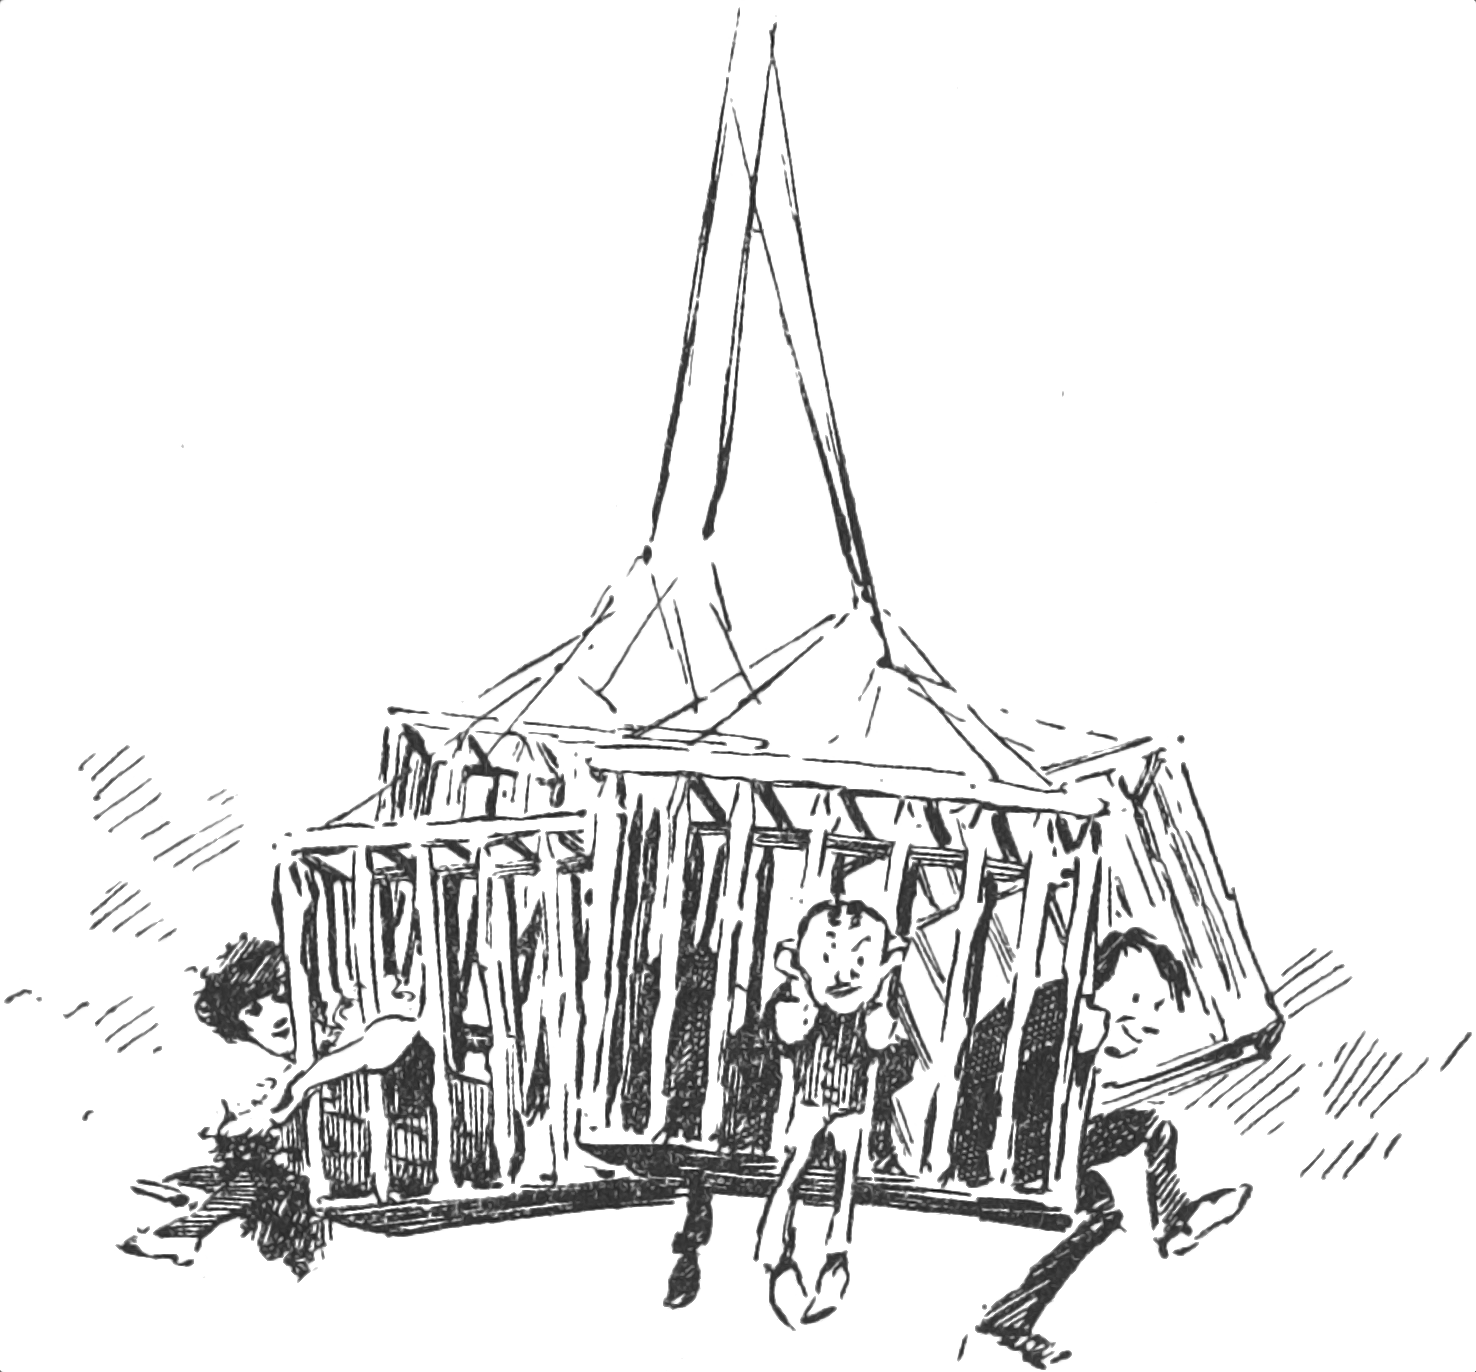
\includegraphics[width=.5\linewidth]{20tailpiece}
%\captionlistentry{Tailpiece to Chapter \thechapter}
\end{figure}